Os algoritmos de inspiração biológica têm sido amplamente utilizados na otimização de ANNs. Baseados em processos biológicos, como o comportamento de enxames de insetos ou a evolução genética, estes algoritmos permitem encontrar soluções eficientes e subótimas em espaços de alta dimensionalidade~\cite{Fister2013AOptimization}\.
Ao aplicá-los na otimização dos parâmetros de ANNs, é possível melhorar o desempenho e a capacidade de generalização destes modelos computacionais, contribuindo para avanços significativos na área de Machine Learning.

\subsection{Algoritmos Evolutivos}\label{subsec:algoritmos-evolutivos}

Em Angeline, et al.~\cite{Angeline1994AnNetworks}, os autores argumentam que os métodos tradicionais de indução de redes neuronais recorrentes (RNN), que assumem uma classe de arquiteturas pré-definidas para cada tarefa, são inadequados, pois as interações entre a estrutura da rede e a sua função não são bem compreendidas, propondo, em alternativa, o uso de algoritmos evolutivos (EA), nomeadamente o programa GNARL, que adquire simultaneamente a estrutura e os pesos das RNNs. O GNARL possibilita a descoberta de comportamentos e topologias complexas que seriam excluídas por métodos convencionais com restrições arquiteturais artificiais, através da pesquisa flexível e dinâmica no espaço de topologias de rede, permitindo modificações estruturais e paramétricas com base na aptidão da rede.
O GNARL promove a emergência da complexidade e comportamento da rede neuronal conforme os requisitos da tarefa, sem impor restrições artificiais, permitindo a descoberta eficiente de soluções adequadas.

\begin{figure}[htbp]
    \centering
    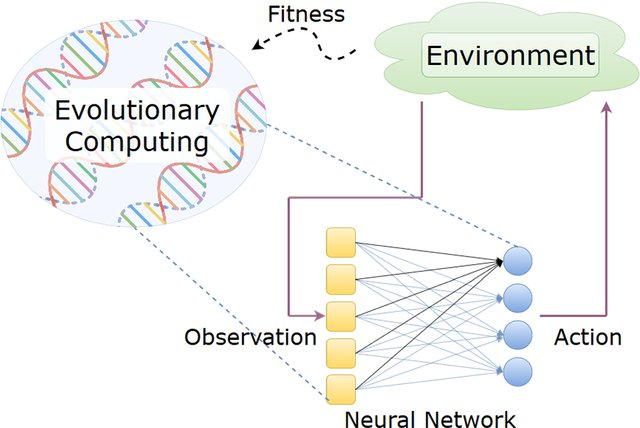
\includegraphics[width=0.48\textwidth]{imagens/evo_alg}
    \caption{Aplicação de algoritmos evolutivos no design de ANNs~\cite{Darwish2020ALearning}}
    \label{fig:evo_alg}
\end{figure}

Em 1995, no seu artigo seminal, Branke~\cite{Branke1995EvolutionaryTraining} aborda a aplicação de algoritmos evolutivos na projeção e treino de redes neuronais, explorando as vantagens e desafios dessa abordagem e destacando a importância de implementações paralelas para lidar com o aumento da complexidade dos problemas reais e a exigência de grande poder computacional.
O foco principal está na utilização de EAs para otimizar o ‘design’ das ANNs, incluindo a determinação da estrutura da rede, a definição dos pesos das conexões e a pesquisa por topologias ótimas.
Ao contrário dos métodos tradicionais baseados em retropropagação de gradientes, os EAs conseguem explorar múltiplas soluções simultaneamente, o que os torna particularmente úteis em situações em que é difícil obter informação do gradiente, como em redes recorrentes, com funções de transferência não diferenciáveis ou critérios de otimalidade não diferenciáveis.

Na revisão detalhada de Castillo, et al.~\cite{Castillo2003ArtificialAlgorithms}, são analisadas as diversas abordagens de projeção de ANNs utilizando algoritmos evolutivos (EAs).
O estudo foca-se especificamente nos operadores genéticos empregados nessas abordagens e identifica três principais estratégias na evolução de ANNs:
\begin{itemize}
    \item Evolução dos pesos das conexões
    \item Evolução da arquitetura da rede
    \item Evolução das regras de aprendizagem
\end{itemize}

Uma das vantagens dos EAs é a capacidade de treinar, simultaneamente, múltiplas redes em processadores separados, graças ao seu paralelismo intrínseco.
Ao contrário dos métodos de otimização convencionais, que tendem a se concentrar em certos parâmetros, os EAs permitem a otimização conjunta da capacidade de aproximação e do tamanho da rede.
Além disso, a incorporação do efeito Baldwin~\cite{Downing2010TheNetworks} nos métodos de evolução de ANNs pode melhorar significativamente a sua eficiência, permitindo a convergência para o ótimo global~\cite{Castillo2003ArtificialAlgorithms}\.
Essas descobertas ressaltam a utilidade e o potencial dos EAs na otimização abrangente e efetiva de ANNs.

\begin{figure}[htbp]
    \centering
    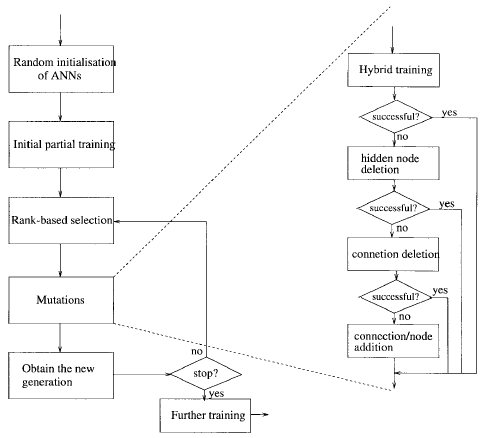
\includegraphics[width=0.48\textwidth]{imagens/evo_alg2}
    \caption{Principais passos do EPNet. Extraído de ~\cite{Yao1997ANetworks}}
    \label{fig:epnet}
\end{figure}

Já em 1997, Yao e Liu~\cite{Yao1997ANetworks} apresentam um novo sistema evolutivo baseado na programação evolutiva de Fogel~\cite{Fogel1990EvolvingNetworks}\, chamado EPNet, para evoluir ANNs. Ao contrário de estudos anteriores, o EPNet coloca ênfase na evolução dos comportamentos das redes, utilizando cinco operadores de mutação, entre os quais, o treino parcial e a divisão de nós.
O EPNet evolui simultaneamente a arquitetura e os pesos das conexões, procurando reduzir o ruído na avaliação de aptidão, para além de promover a \qq{economia} das redes evoluídas, preferindo a exclusão à adição de nós/conexões.
As experiências realizadas com o EPNet em vários problemas de referência mostram que o sistema não só consegue produzir redes muito compactas, com boa capacidade de generalização, face a outros algoritmos, como permite a exploração eficiente do espaço de pesquisa, graças à sua pesquisa global, algo difícil de implementar manualmente.
No entanto, o EPNet pode exigir tempos de computação mais longos dado a dimensão do espaço de pesquisa, tornando-o mais adequado para aplicações onde o tempo de projeto e treino da rede não é crítico.

\begin{figure}[htbp]
    \centering
    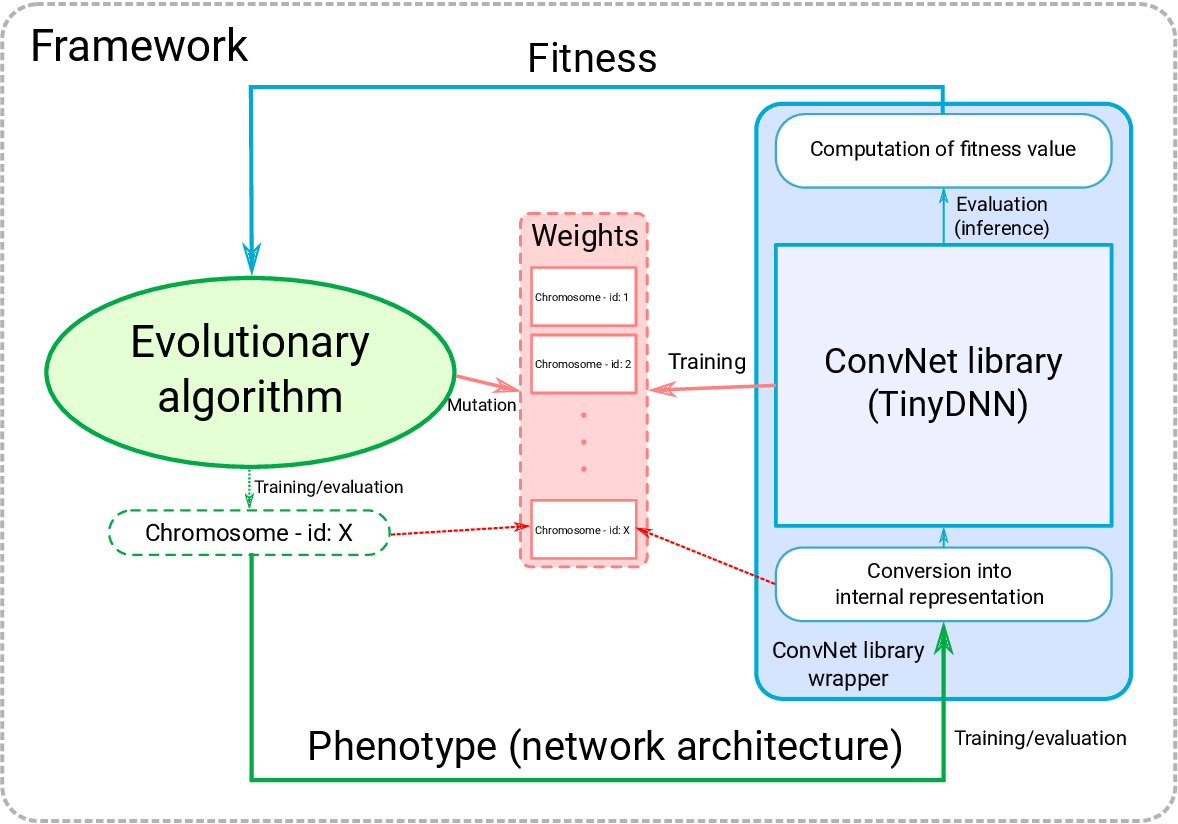
\includegraphics[width=0.48\textwidth]{imagens/evo_alg3}
    \caption{Aplicação de algoritmos evolutivos em redes convolucionais\cite{Badan2019EvolutionaryDesign}}
    \label{fig:evo_alg_cnn}
\end{figure}

Também no campo da evolução computacional (EC), algoritmos inovadores têm sido desenvolvidos para otimizar ANNs. Rocha, et.
al~\cite{Rocha2007EvolutionRegression}, apresentam duas abordagens distintas: a evolução de topologias neuronais e a otimização simultânea de topologias e pesos.
Os algoritmos propostos utilizam uma representação direta e uma mutação estrutural para adicionar ou remover conexões e pesos das redes, recorrendo a técnicas de \textit{model ensemble} para criar modelos mais precisos a partir dos melhores modelos obtidos durante a evolução.
No caso da otimização simultânea, os pesos das conexões são otimizados por meio de uma evolução Lamarckiana, combinando mutações aleatórias com um algoritmo de pesquisa local baseado em gradientes.
Os resultados experimentais mostram que essas abordagens superam outros algoritmos de mineração de dados e métodos heurísticos de seleção de ANNs.

Extreme Learning Machine (ELM)~\cite{Guang-BinHuang2004ExtremeNetworks} é um algoritmo de aprendizagem para redes neuronais de camada única (SLFN), que se destaca pela sua velocidade de treino.
Apesar da sua rapidez e eficiência, o ELM pode exigir um número maior de neurónios ocultos, devido à determinação aleatória dos pesos de entrada e dos \textit{biases} ocultos.

\begin{figure}[htbp]
    \centering
    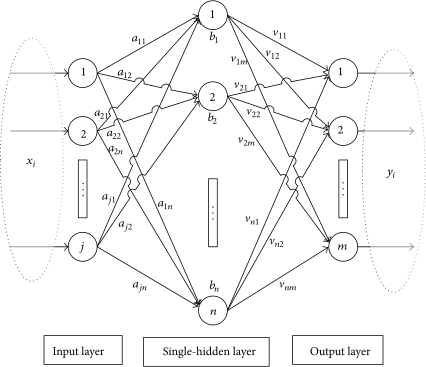
\includegraphics[width=0.48\textwidth]{imagens/slfn}
    \caption{Estrutura de uma SLFN~\cite{Erdem2020IntroductionMachines}}
    \label{fig:slfn}
\end{figure}

Para corrigir este problema, Zhu, et al.~\cite{Zhu2005EvolutionaryMachine}, propuseram um algoritmo híbrido chamado E-ELM, que utiliza a evolução diferencial~\cite{Storn1997DifferentialSpaces} para selecionar os pesos de entrada, e a inversa generalizada de Moore-Penrose para determinar analiticamente os pesos de saída.
Os resultados experimentais mostram que o E-ELM, geralmente, alcança um desempenho de generalização mais elevado do que outros algoritmos, como a retropropagação e o ELM. Além disso, o E-ELM consegue obter arquiteturas de rede mais compactas em comparação com o ELM, aumentando a velocidade de resposta, algo particularmente útil em aplicações que requerem uma resposta rápida a dados desconhecidos.

\subsection{Algoritmos Genéticos}\label{subsec:ga}

Os algoritmos genéticos (GA) são algoritmos de pesquisa baseados na mecânica da seleção natural e nos princípios da genética, que combinam a sobrevivência dos indivíduos mais aptos numa população de entidades binárias - cromossomas, com a troca estruturada e aleatória de informação (Fig.~\ref{fig:ea_flowchart}). Em cada geração, um novo conjunto de indivíduos (sequências) é criado usando pedaços dos elementos mais aptos.
Ainda que aleatórios, os algoritmos genéticos não são uma simples \qq{caminhada} estocástica, explorando eficientemente a informação histórica para especular novos pontos de pesquisa com um desempenho esperado melhorado~\cite{Goldberg1989GeneticLearning}.

\begin{figure}[htbp]
    \centering
    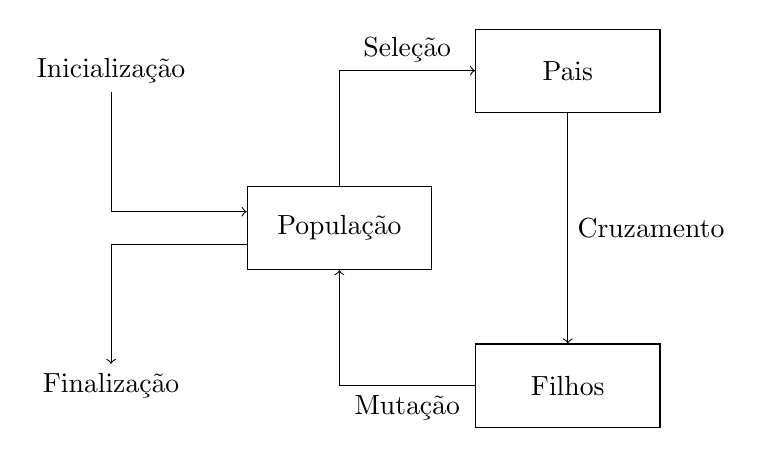
\begin{tikzpicture}[node distance = 2.9cm]
        \tikzstyle{frame} = [rectangle, draw, text width=6em, text centered, minimum height=3em]
        \tikzstyle{line} = [draw, ->]
        \node [frame] (pop) {População};
        \node [above=2cm, left of=pop] (init) {Inicialização};
        \node [below=2cm, left of=pop] (term) {Finalização};
        \node [frame, above=2cm, right of=pop] (parents)  {Pais};
        \node [frame, below=2cm, right of=pop] (off)  {Filhos};
        \path [line] (parents) -- node[right,align=left,pos=.5] {Cruzamento}(off);
        \path [line] (init) |- (pop.170);
        \path [line] (pop.190) -| (term);
        \path [line] (off) -| node[below,pos=.25, align=center] {Mutação}(pop);
        \path [line] (pop) |- node[above,pos=.75, align=center] {Seleção}(parents);
    \end{tikzpicture}
    \caption{Processo geral de um algoritmo genético}
    \label{fig:ea_flowchart}
\end{figure}

A crescente popularidade das ANNs na década de 80 potenciou o surgimento de novas técnicas para o seu treino e otimização, com particular atenção para os algoritmos genéticos.
A retropropagação (BP), apesar da sua utilidade e simplicidade, apresentava limitações, entre as quais:
\begin{itemize}
    \item a pobre escalabilidade face ao aumento da complexidade do problema (maior dimensionalidade e/ou complexidade dos dados), resultando numa degradação de desempenho
    \item a necessidade de diferenciabilidade no cálculo dos gradientes, que impede o seu uso em certos tipos de nós e critérios de otimização não diferenciáveis (ND).
\end{itemize}

Para superar essas limitações, Montana e Davis~\cite{Montana1989} propuseram um algoritmo genético capaz de codificar os pesos duma rede neuronal \textit{feed-forward} (FNN) numa lista de números reais, utilizando uma função de \textit{fitness} para avaliar o desempenho da rede, e incorporando operadores de mutação, cruzamento e gradiente para gerar novas soluções.
Os autores realizaram múltiplas experiências usando uma base de dados de imagens de energia acústica, e compararam o desempenho do GA com o do BP. Os resultados mostraram que o GA superou o BP em termos de velocidade de treino e capacidade de lidar com tipos de nós e critérios de otimização, provando os GAs como uma alternativa eficaz à retropropagação, especialmente em problemas complexos e não diferenciáveis.

O uso das redes neuronais pelas empresas como ferramentas de análise e resolução de problemas era cada vez mais popular no final da década de 90, dada a sua capacidade de aproximar funções desconhecidas com precisão.
No entanto, as técnicas de otimização baseadas em gradiente, como a retropropagação, têm limitações na busca de soluções globais.

Segundo Sexton, et al.~\cite{Sexton1998, Sexton1999}, essas limitações podem resultar em desempenho inconsistente e imprevisível.
Por outro lado, a imposição de restrições no espaço de pesquisa e a reestruturação da arquitetura da rede não era necessária, desde que fossem utilizados uma arquitetura inicial suficientemente complexa e um algoritmo global apropriado, apresentando como alternativa os algoritmos genéticos, que oferecem vantagens na obtenção de soluções mais robustas.
Os autores também apresentam um estudo de Monte Carlo que compara o desempenho de várias técnicas de pesquisa global, incluindo o Simulated Annealing (SA) e o GA, no qual mostram que o GA conseguiu obter soluções mais robustas, sem a necessidade de impor restrições no espaço de pesquisa ou reestruturar a arquitetura da rede, destacando a sua importância como uma ferramenta versátil de estimativa de funções.

\begin{table}[htbp]
    \centering
    \caption{Resultados do problema do cancro da mama\cite{Sexton1999}}
    \begin{tabular}{cccc}
        \hline
        Algoritmo & GA      & SA      & BP        \\ \hline
        Classificação     & 98.5\%  & 97.2\%  & 97.2\%    \\
        Erro tipo-1       & 1.5\%   & 3.1\%   & 2.3\%     \\
        Erro tipo-2       & 1.4\%   & 1.6\%   & 4.1\%     \\
        N.º de avaliações & 100.000 & 493.535 & 1.174.000 \\
        Tempo de CPU (em s)
        & 618     & 4.812   & 497       \\ \hline
    \end{tabular}
    \label{tab:breastcancer}
\end{table}

Já em Whitley, et al.~\cite{Whitley1990}\, os autores propõem a aplicação de algoritmos genéticos em problemas de NNs, incluindo a otimização dos pesos das conexões em FNNs, mas também na descoberta de novas arquiteturas de conectividade que aprendem usando a propagação de erros.
Os resultados das suas experiências indicam que a pesquisa genética pode ser competitiva com o algoritmo de \textit{backpropagation} e oferecer vantagens em termos de flexibilidade e escalabilidade.
Além disso, a combinação de algoritmos genéticos com outras técnicas de otimização, como Hill Climbing, pode aumentar a eficiência da pesquisa.

\begin{figure}[htbp]
    \centering
    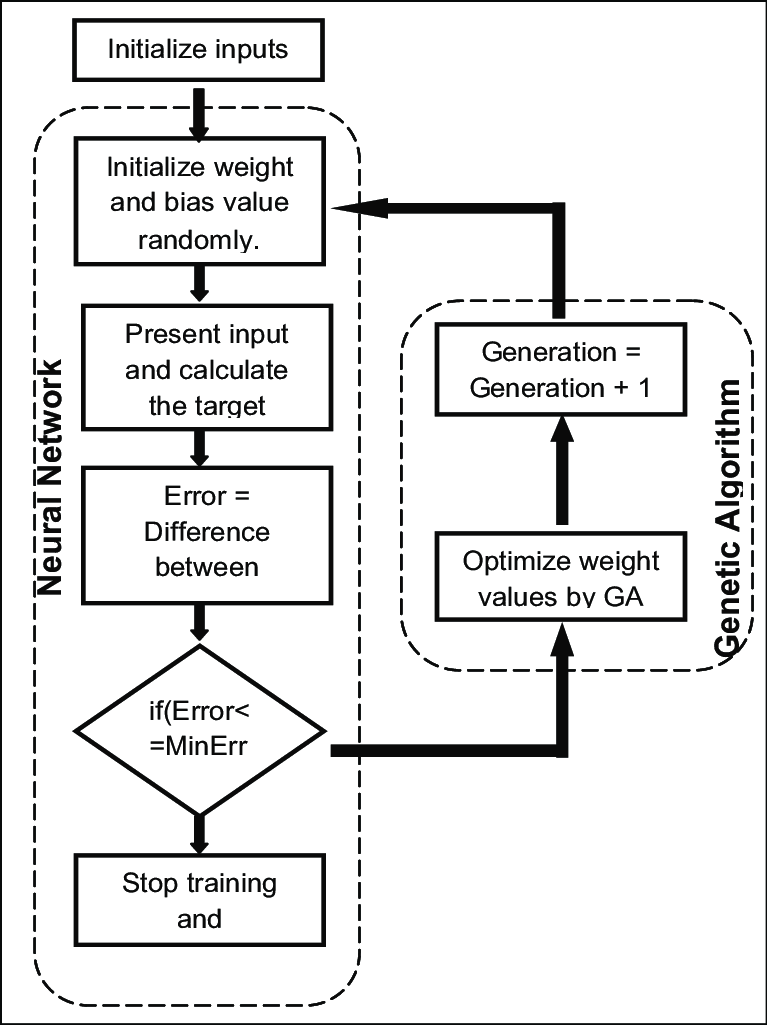
\includegraphics[width=0.4\textwidth]{imagens/ga_nn}
    \caption{Otimização de uma rede neuronal com um algoritmo genético~\cite{Rahman2015AnAlgorithms}}
    \label{fig:ga_nn}
\end{figure}

Em 1994, Maniezzo~\cite{Maniezzo1994} apresenta um sistema baseado num algoritmo genético paralelo, utilizado para evoluir FNNs em duas áreas distintas: a aprendizagem de funções booleanas e o controlo de robôs.
O sistema proposto, intitulado de ANNA ELEONORA, reduz a granularidade da codificação e topologia da rede, permitindo a rápida identificação de distribuições promissoras de pesos e aumentando a eficiência da pesquisa no espaço de soluções, e utiliza um operador genético cooperativo de otimização local para melhorar a exploração das soluções encontradas.
Os resultados obtidos demonstraram que o sistema consegue evoluir as redes neuronais com bom desempenho em ambos os domínios, desempenho esse superior à obtida com o algoritmo de retropropagação.

Mais recentemente, David e Greental~\cite{David2014GeneticNetworks} apresentam uma abordagem que utiliza algoritmos genéticos para melhorar o desempenho de autoencoders profundos, através da otimização dos pesos das camadas ocultas.
Autoencoders~\cite{Pierre2011} são redes neuronais não supervisionadas que aprendem a codificar dados de entrada numa representação de menor dimensão - o espaço latente, e a descodificar essa representação nos dados de saída.
Os autores avaliaram o desempenho do método numa tarefa de reconhecimento de dígitos manuscritos, recorrendo ao dataset MNIST, concluindo que a abordagem assistida pelo GA conseguiu produzir autoencoders com menor erro de reconstrução e maior precisão de classificação, revelando-se uma alternativa eficaz para treinar redes neuronais profundas.